\chapter{Metodologia}
\label{cap:metodologia}
O sistema proposto neste projeto, se refere a uma plataforma que fornece tanto os dispositivos para a captação dos dados dos imunobiológicos, quanto ao sistema em nuvem para armazenagem dos dados e de um aplicativo móvel para a gerência e análise das informações, seguindo a mesma estrutura representada na figura \ref{fig:end-nodes-gateways}, de modo a fornecer aos usuários, um produto  de fácil uso para monitorização de temperatura e umidade, possibilitando o histórico dos dados coletados em um determinado cliente.

Podemos então, separar este sistema em quatro partes, cada uma delas com uma determinada função, elas são, end-node, gateway, servidor e aplicativo móvel.

% ---
\section{End node}
\label{metod:node}
Dentre os diversos sensores disponíveis no mercado para monitoramento de temperatura e umidade, optou-se por escolher um sensor da família DHT, pois é bastante difundida na comunidade, tendo uma boa relação custo benefício. Entre esses sensores, aderimos por usar o DHT22, que consegue captar a temperatura e umidade do ambiente dentro das faixas necessárias para o projeto, com uma boa precisão.

% ---
\section{Gateway}
\label{metod:gateway}

% ---
\section{Servidor}
\label{metod:servidor}
Para este projeto, o servidor tem as seguintes responsabilidades: armazenar os dados coletados pelos end-nodes, juntamente com os dados do instituto que está usando a aplicação e dos seus respectivos end-nodes e gateways adquiridos; fornecer rotas para troca de informações com o aplicativo e o gateway, para que possam realizar sua devidas funções.

% ---
\subsection{Padrões de projetos}
\label{metod:servidor:padroes}
Foi escolhido para desenvolver o servidor, a utilização do Node.js e a linguagem Typescript, se baseando em alguns padrões de softwares, como o Domain-Driven Design (DDD), Test-Driven Development (TDD) e o SOLID visando assim, a construção de um servidor robusto, escalável e de fácil manutenção.

Vale salientar que, esses padrões de softwares, são metodologias de desenvolvimento, e devem ser aplicados de acordo com a demanda da aplicação em construção. Elas são boas práticas, entretanto, dependendo do projeto, alguns pontos podem acabar deixando o processo lendo, e dando pouco benefício, e por isso, nesse projeto, não foi seguido fielmente esses padrões, apenas foi baseado.

Antes de tudo, é preciso definir as regras de negócio básicas do servidor, elas servem para garantir que a aplicação atenda as necessidades esperadas. Para este serviço deve ser possível o usuário se cadastrar, para assim realizar seu \textit{login}, e ter acesso às funcionalidades de cadastrar, editar e remover seus end nodes e seus gateways, além de poder visualizar os dados coletados.

Durante o desenvolvimento de um software, é essencial que a entrega do software funcione corretamente, com qualidade e de acordo com as regras de negócio. Para garantir tais exigências, é importante que se realize testes, tendo em vista identificar possíveis erros antes de chegar aos usuários. Entretanto, realizar testes corretamente é uma tarefa complicada, por isto, existem diversas metodologias, objetivamente facilitar e simplificar os testes dos diferentes componentes de um produto. O TDD é uma dessas metodologias, ela defende o desenvolvimento do teste antes das funcionalidades, garantindo a cobertura completa do código pelos testes.

Junto com o TDD, foi utilizado também o DDD, uma filosofia para auxiliar os desenvolvedores na construção de aplicações complexas de software, ela é referência na organização do código, separando por domínios, de forma isolada. Para poder implementar bem o DDD é preciso definir quais são os domínios da aplicação, analisando as regras de negócio, foi separado em três domínios: end nodes, gateways e usuários.

É preciso também, separar a camada de domínio da aplicação da camada de infraestrutura, a camada de infraestrutura é responsável pelas tecnologias utilizadas para realizar determinada função, por exemplo, a camada de domínio sabe que precisa armazenar os dados dos sensores, mas não é precisar saber onde e nem como, isso é de responsabilidade da camada de infraestrutura.

Para ter uma melhor separação das responsabilidades entre as camadas, é comum utilizar o DDD junto com princípios do SOLID. O SOLID é um acrônimo de 5 princípios da programação orientada a objetos que ajudam o programador a escrever códigos mais limpos, com alta manutenibilidade, separando as responsabilidades e diminuindo acoplamentos.

% ---
\subsection{Banco de dados}
\label{metod:servidor:db}
É preciso armazenar os dados coletados pelos sensores, para futuras consultas, os dados de transmissão dos pacotes, para utilizar se houver perdas entre as transmissões, e é preciso também, salvar os dados dos usuários e dos seus respectivos produtos cadastrados na plataforma. Tais dados têm suas diferenças, e por isto foi escolhido utilizar banco de dados diferentes para cada um deles.
	
Começando pelos dados coletados pelos sensores e transmitido pelos end-nodes, esses dados são de medidas, coletados com um período curto, e consequentemente, possuem um grande volume. Por isto, foi escolhido utilizar o InfluxDB para armazenar tais dados.

Foi criado duas \textit{measurements} dentro do banco, uma referente aos dados dos sensores e outra aos dados do pacote transmitido, os dois possuindo a mesma  \textit{tag}, o identificador do end node, chamado de endnodeId. Dentro da medida Sensor, foi adicionado dois campos referente a temperatura e umidade do ambiente. Para a medida Package, foi adicionado os campos success, rssi e snr, atributos necessários para saber se o pacote foi entregue com sucesso, a dificuldade de transmitir esse pacote e a relação sinal-ruído. Podemos então ver uma representação do banco na figura \ref{fig:influxdb-model}.

\begin{figure}[H]
  \centering
  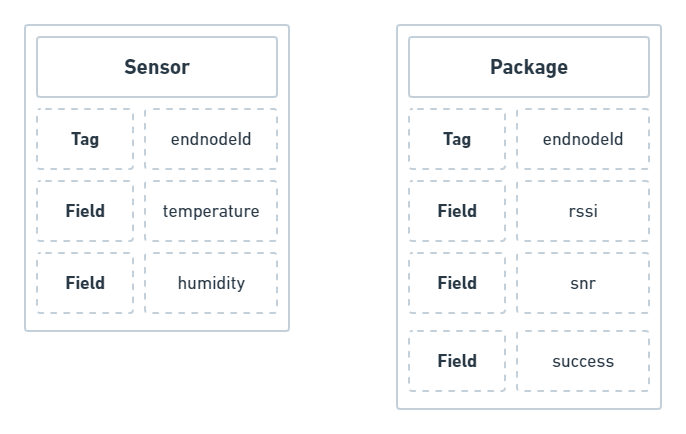
\includegraphics[width=.80\textwidth]{assets/influx-model.png} 
  \caption{Medidados dento do banco de dados InfluxDB \todo{refazer esse modelo} (autoral).}
  \label{fig:influxdb-model} 
\end{figure}

Diferentes dos dados que vem dos hardwares, as informações dos usuários e seus dispositivos, não possuem essa demanda alta de escrita e leitura, e mais importante, contém relações entre eles, o que torna banco de dados relacionais uma boa opção para armazenar tais dados. Entre tantos bancos de dados relacionais, foi optado por usar o PostgreSQL por motivos de afinidade.

Cada usuário pode possuir inúmeras gateways e end nodes cadastrados, e cada end node precisa ser vinculado com apenas um gateway. Essas relações entre entre as entidades no postgres representada na figura \ref{fig:postgres-model}, foi pensada olhando tanto para os cenários de pequenos postos de saúde, que tem apenas um local para armazenar seus imunobiológicos, quando para grande hospitais e laboratórios, que pode tem varias salas, com dada sala contendo uma ou mais equipamentos frigoríficos.

\begin{figure}[H]
  \centering
  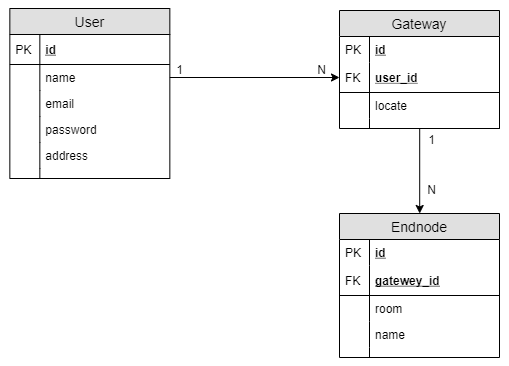
\includegraphics[width=.80\textwidth]{assets/postgres-model.png} 
  \caption{Modelo entidade relacionamento do PostgreSQL (autoral).}
  \label{fig:postgres-model} 
\end{figure}

% ---
\subsection{Containers}
\label{metod:servidor:containers}


% ---
\subsection{Deploy}
\label{metod:servidor:deploy}

% ---
\section{Aplicativo móvel}
\label{metod:app}